\subsection{Herança}

Neste capítulo serão definidos os princípios da herança, sendo que, são eles que
permitem que a programação orientada a objetos seja considerada tão poderosa.

Segundo \citeonline{programmingInObjectiveC}, através deste conceito você poderá
construir uma classe com base em uma outra classe já existente e personalizá-la
de acordo com a regra de negócio exigida pela sua aplicação.

Na Figura \ref{fig:heranca}, tem-se a sintaxe da utilização da herança
implementado na linguagem \acs{PHP}:

\begin{figure}[h!tb]
	\caption{Herança na linguagem PHP}
	\label{fig:heranca}

	\centering
	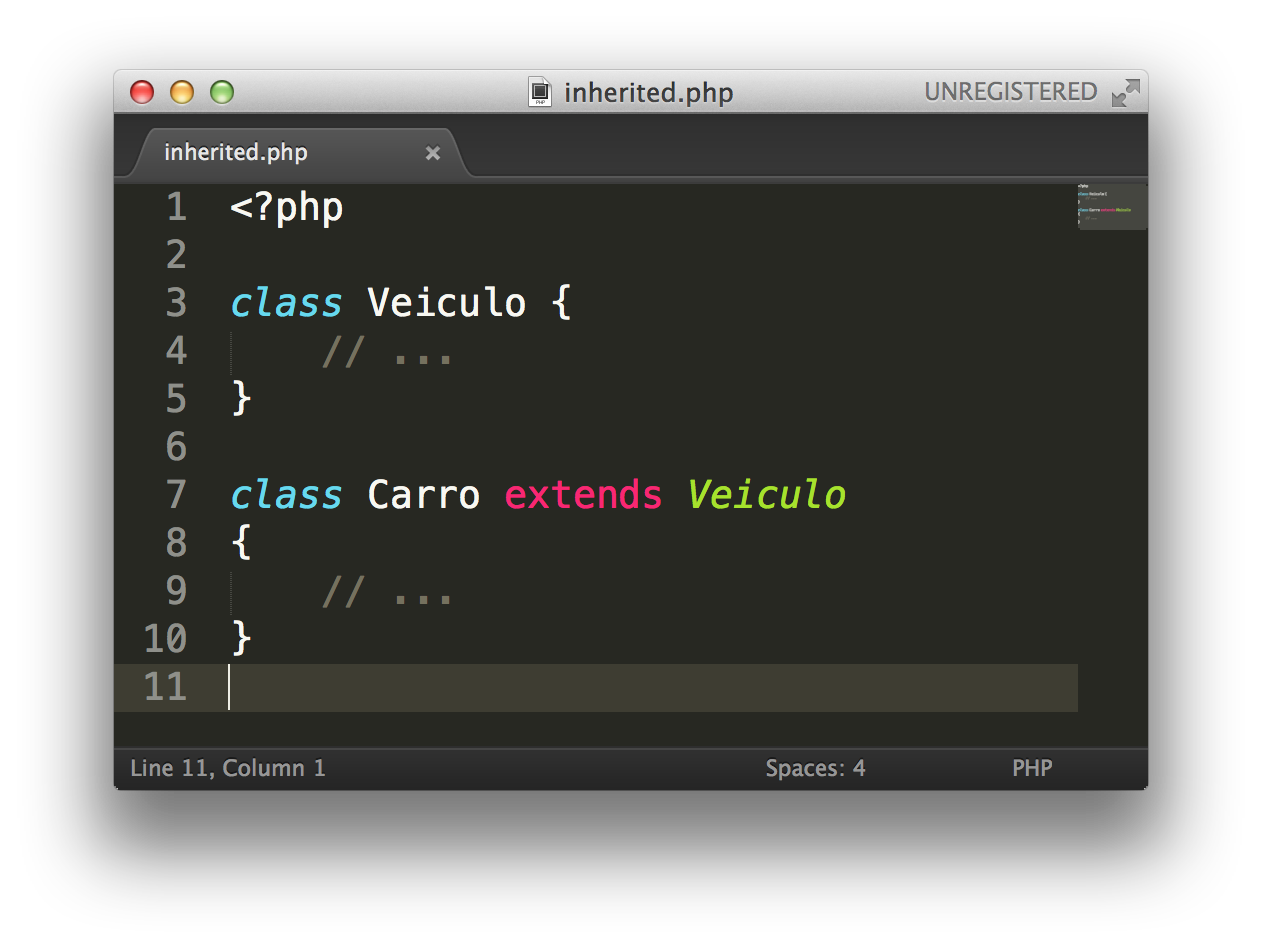
\includegraphics[width=0.75\textwidth]{images/inherited.png}

	\centering
	\footnotesize Fonte: \fonteOAutor
\end{figure}

\FloatBarrier 	% Este comando impede que as imagens
				% flutuem a partir deste ponto no seu documento

A seguir, é apresentado em detalhes as linhas de código exibidas na Figura
\ref{fig:heranca}:

\begin{alineas}
    \item linha 3: definição da classe base \textit{Veiculo};
    \item linha 7: cria-se a classe filha \textit{Carro} com base na classe
    \textit{Veiculo}.
\end{alineas}

Uma vez definido o conceito de herança, a seguir será abordardado outro conceito
da orientação a objetos, o polimorfismo.
